\documentclass[11pt,a4paper]{article}

% ── Geometry ──
\usepackage[top=2.5cm, bottom=2.5cm, left=2.5cm, right=2.5cm]{geometry}

% ── Fonts ──
\usepackage[T1]{fontenc}
\usepackage{helvet}
\renewcommand{\familydefault}{\sfdefault}

% ── Colors ──
\usepackage[table]{xcolor}
\definecolor{accentblue}{HTML}{4A7BF7}
\definecolor{headerblue}{HTML}{4472C4}
\definecolor{darktext}{HTML}{1A1A1A}
\definecolor{ruleblue}{HTML}{4472C4}

% ── Packages ──
\usepackage{enumitem}
\usepackage{array}
\usepackage{booktabs}
\usepackage{tabularx}
\usepackage{tikz}
\usetikzlibrary{shapes.geometric, arrows.meta, positioning}
\usepackage{hyperref}
\usepackage{parskip}
\usepackage{titlesec}
\usepackage{fancyhdr}
\usepackage{needspace}

% ── Paragraph spacing ──
\setlength{\parskip}{0.5em plus 0.15em minus 0.1em}
\setlength{\parindent}{0pt}

% ── Page style ──
\pagestyle{fancy}
\fancyhf{}
\renewcommand{\headrulewidth}{0pt}
\fancyfoot[C]{\thepage}

% ── Section formatting ──
\titleformat{\section}
  {\Large\bfseries\color{darktext}}
  {\thesection.}{0.5em}{}
  [\vspace{-0.2em}{\color{ruleblue}\hrule height 2pt}]

\titleformat{\subsection}
  {\large\bfseries\color{accentblue}}
  {}{0em}{}

\titlespacing*{\section}{0pt}{1.8em}{1em}
\titlespacing*{\subsection}{0pt}{1.2em}{0.6em}

% ── Custom list with dashes ──
\setlist[itemize]{label=---, leftmargin=2em, itemsep=4pt, parsep=1pt, topsep=5pt}

% ── Table style macros ──
\newcommand{\tableheadercolor}{\rowcolor{headerblue}}
\newcommand{\tableheaderfont}{\color{white}\bfseries}

% ── Hyperref ──
\hypersetup{
    colorlinks=true,
    linkcolor=accentblue,
    urlcolor=accentblue,
}

\color{darktext}

\begin{document}

% ══════════════════════════════════════════════════════════════
% TITLE
% ══════════════════════════════════════════════════════════════

\begin{flushleft}
{\small\color{accentblue}\textbf{MILESTONE 2\;\;$\cdot$\;\;PROJECT REPORT}}\\[0.5em]
{\fontsize{24}{29}\selectfont\bfseries AI Real Estate Advisory \& Agentic AI\\[0.15em] Property Advisor}
\end{flushleft}

\vspace{1.8em}

% ══════════════════════════════════════════════════════════════
% 1. INTRODUCTION & PROBLEM STATEMENT
% ══════════════════════════════════════════════════════════════

\section{Introduction \& Problem Statement}

Bengaluru's real estate market has over 1,200 active localities and thousands of property listings, making manual valuation and investment analysis infeasible. While Milestone~1 demonstrated that a classical ML model (Linear Regression) can predict property prices from structured data, it suffers from fundamental limitations:

\begin{itemize}
    \item No contextual market understanding
    \item Static dataset with no dynamic knowledge retrieval
    \item No reasoning or recommendation capability
    \item No multi-source synthesis for investment advisory
\end{itemize}

\vspace{0.2em}
\textbf{Core Problem (Milestone 2): Design an autonomous AI agent that can:}

\begin{itemize}
    \item Predict property prices using a trained ML model
    \item Retrieve relevant market insights dynamically via RAG
    \item Perform multi-step reasoning using an LLM
    \item Generate structured investment advisory reports
\end{itemize}

% ══════════════════════════════════════════════════════════════
% 2. SYSTEM EVOLUTION
% ══════════════════════════════════════════════════════════════

\section{System Evolution\;\;(Milestone 1 $\rightarrow$ Milestone 2)}

\vspace{0.6em}
\begin{tabularx}{\textwidth}{>{\raggedright\arraybackslash}p{2.8cm}
                              >{\raggedright\arraybackslash}X
                              >{\raggedright\arraybackslash}X}
\tableheadercolor
\tableheaderfont Component & \tableheaderfont Milestone 1 & \tableheaderfont Milestone 2 \\
\midrule
Data          & Static Bengaluru CSV dataset   & RAG knowledge base (ChromaDB)    \\[5pt]
Retrieval     & None (direct feature input)    & Semantic search (HuggingFace)    \\[5pt]
Prediction    & Linear Regression only         & ML + LLM reasoning               \\[5pt]
Output        & Numeric price (Lakhs)          & Structured advisory report        \\[5pt]
Pipeline      & Single-step prediction         & Multi-step agentic workflow        \\[5pt]
Capability    & Price estimation               & Valuation + Reasoning + Advisory   \\
\bottomrule
\end{tabularx}

% ══════════════════════════════════════════════════════════════
% 3. SYSTEM ARCHITECTURE
% ══════════════════════════════════════════════════════════════

\newpage

\section{System Architecture\;\;(Agent-Based)}

The system is redesigned as a multi-layer agent architecture. Each layer has a clearly defined responsibility, enabling modular development and controlled reasoning.

\subsection{Layers}

\begin{itemize}
    \item 1.\;Input Layer --- User property details via Streamlit UI (location, sqft, BHK, bath, balcony, area type, availability)
    \item 2.\;Agent Layer (LangGraph) --- Controls execution flow via \texttt{StateGraph}, maintains typed state (\texttt{AgentState}), enables sequential node execution
    \item 3.\;Prediction Layer --- ML model inference using pre-trained Linear Regression with StandardScaler
    \item 4.\;Retrieval Layer --- Semantic search over market knowledge base via ChromaDB + all-MiniLM-L6-v2
    \item 5.\;Generation Layer --- Google Gemini 1.5 Pro generates structured advisory report
    \item 6.\;Output Layer --- Formatted report with valuation, comps, recommendation, disclaimer
\end{itemize}

\subsection{Flow Diagram}

\vspace{0.8em}
\begin{center}
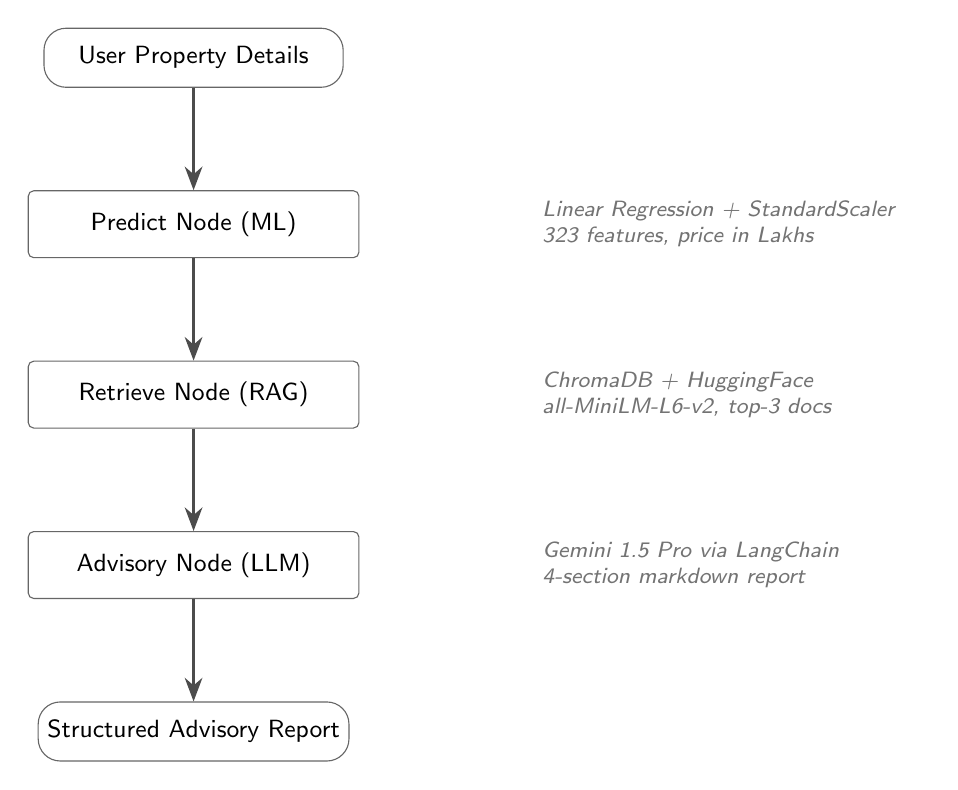
\begin{tikzpicture}[
    node distance=1.3cm,
    every node/.style={font=\small},
    process/.style={rectangle, draw=black!60, fill=white, minimum width=4.2cm, minimum height=0.85cm, rounded corners=2pt},
    io/.style={rectangle, draw=black!60, fill=white, rounded corners=8pt, minimum width=3.8cm, minimum height=0.75cm},
    arrow/.style={-{Stealth[length=3mm]}, thick, black!70}
]

\node[io] (input) {User Property Details};
\node[process, below=of input] (predict) {Predict Node (ML)};
\node[process, below=of predict] (retrieve) {Retrieve Node (RAG)};
\node[process, below=of retrieve] (advisory) {Advisory Node (LLM)};
\node[io, below=of advisory] (output) {Structured Advisory Report};

\draw[arrow] (input) -- (predict);
\draw[arrow] (predict) -- (retrieve);
\draw[arrow] (retrieve) -- (advisory);
\draw[arrow] (advisory) -- (output);

% Side annotations
\node[right=2.2cm of predict, text width=4.8cm, font=\footnotesize\itshape, text=black!55] {Linear Regression + StandardScaler\\323 features, price in Lakhs};
\node[right=2.2cm of retrieve, text width=4.8cm, font=\footnotesize\itshape, text=black!55] {ChromaDB + HuggingFace\\all-MiniLM-L6-v2, top-3 docs};
\node[right=2.2cm of advisory, text width=4.8cm, font=\footnotesize\itshape, text=black!55] {Gemini 1.5 Pro via LangChain\\4-section markdown report};

\end{tikzpicture}
\end{center}

% ══════════════════════════════════════════════════════════════
% 4. AGENT PIPELINE
% ══════════════════════════════════════════════════════════════

\newpage

\section{Agent Pipeline --- Step by Step}

\vspace{0.6em}
\begin{tabularx}{\textwidth}{>{\centering\arraybackslash}p{1cm}
                              >{\raggedright\arraybackslash}p{3.5cm}
                              >{\raggedright\arraybackslash}X}
\tableheadercolor
\tableheaderfont Step & \tableheaderfont Action & \tableheaderfont Detail \\
\midrule
1 & Property Input       & User provides location, sqft, BHK, bathrooms, balconies, area type, availability via Streamlit form \\[6pt]
2 & State Initialization & \texttt{AgentState} TypedDict created with property details and API key \\[6pt]
3 & Price Prediction     & \texttt{predict\_node} builds 323-dim feature vector, applies StandardScaler, runs Linear Regression \\[6pt]
4 & Market Retrieval     & \texttt{retrieve\_node} queries ChromaDB with location-specific prompt, returns top-3 semantic matches \\[6pt]
5 & LLM Advisory         & \texttt{generate\_advisory\_node} invokes Gemini 1.5 Pro with structured prompt template (4 sections) \\[6pt]
6 & Report Display       & Streamlit renders price card, metrics grid, markdown report, and action badge \\
\bottomrule
\end{tabularx}

\vspace{1.5em}

% ══════════════════════════════════════════════════════════════
% 5. CORE COMPONENTS (NODE-LEVEL)
% ══════════════════════════════════════════════════════════════

\section{Core Components\;\;(Node-Level)}

\vspace{0.6em}
\begin{tabularx}{\textwidth}{>{\raggedright\arraybackslash}p{4cm}
                              >{\raggedright\arraybackslash}X}
\tableheadercolor
\tableheaderfont Node & \tableheaderfont Function \\
\midrule
\texttt{predict\_node}             & Load \texttt{model.pkl}, \texttt{scaler.pkl}, \texttt{feature\_columns.pkl}; encode inputs into 323-dim vector; scale and predict price in Lakhs \\[8pt]
\texttt{retrieve\_node}            & Initialize ChromaDB with HuggingFace embeddings (all-MiniLM-L6-v2); semantic search on 9 curated market insight documents; return top-3 matches \\[8pt]
\texttt{generate\_advisory\_node}  & Authenticate with Google API; construct \texttt{PromptTemplate} with 4 required sections; invoke Gemini 1.5 Pro via LangChain; return structured markdown \\[8pt]
\texttt{AgentState}                & Typed state container --- \texttt{property\_details}, \texttt{predicted\_price}, \texttt{market\_insights}, \texttt{final\_report}, \texttt{google\_api\_key} \\[8pt]
\texttt{create\_workflow}          & Assembles \texttt{StateGraph}, registers nodes, defines edges (START $\rightarrow$ predict $\rightarrow$ retrieve $\rightarrow$ advisory $\rightarrow$ END), compiles graph \\
\bottomrule
\end{tabularx}

% ══════════════════════════════════════════════════════════════
% 6. LLM REASONING
% ══════════════════════════════════════════════════════════════

\newpage

\section{LLM Reasoning}

Unlike Milestone~1, this system uses LLM-based reasoning via Google Gemini 1.5 Pro. This unlocks capabilities that a classical ML regression model cannot provide --- contextual understanding, natural language generation, and structured advisory output.

\vspace{0.6em}
\begin{tabularx}{\textwidth}{>{\raggedright\arraybackslash}p{2.8cm}
                              >{\raggedright\arraybackslash}X
                              >{\raggedright\arraybackslash}X}
\tableheadercolor
\tableheaderfont Aspect & \tableheaderfont Milestone 1 & \tableheaderfont Milestone 2 \\
\midrule
Output     & Numeric price prediction       & Generated advisory report with 4 structured sections  \\[5pt]
Reasoning  & None (statistical model only)  & Multi-step: predict $\rightarrow$ retrieve $\rightarrow$ reason $\rightarrow$ report \\[5pt]
Pipeline   & Static single-step             & Dynamic agentic workflow (LangGraph)                   \\[5pt]
Knowledge  & Training data only             & RAG-augmented with curated market insights              \\
\bottomrule
\end{tabularx}

\vspace{0.6em}

The LLM prompt enforces four structured sections: (1)~Property Valuation \& Market Summary, (2)~Comparable Property Analysis, (3)~Action Recommendation (INVEST / HOLD / CAUTION), and (4)~Financial \& Legal Disclaimer. This template-based approach mitigates hallucination by constraining output format and grounding the response in retrieved market insights.

% ══════════════════════════════════════════════════════════════
% 7. EVALUATION & RESULTS
% ══════════════════════════════════════════════════════════════

\section{Evaluation \& Results}

\subsection{ML Model Performance (Milestone 1)}

\vspace{0.4em}
\begin{tabularx}{\textwidth}{>{\raggedright\arraybackslash}p{4cm}
                              >{\centering\arraybackslash}X
                              >{\centering\arraybackslash}X}
\tableheadercolor
\tableheaderfont Metric & \tableheaderfont Train & \tableheaderfont Test \\
\midrule
R\textsuperscript{2} Score  & 0.7225 & 0.6949  \\[4pt]
RMSE (Lakhs)                & 62.60  & 67.72   \\[4pt]
MAE (Lakhs)                 & 31.57  & 32.15   \\[4pt]
MAPE (\%)                   & 33.72  & 33.62   \\[4pt]
5-Fold CV Mean              & \multicolumn{2}{c}{0.6980 $\pm$ 0.0107} \\
\bottomrule
\end{tabularx}

\subsection{Agentic System Evaluation (Milestone 2)}

Since the advisory system generates natural language reports, evaluation is qualitative and based on:

\begin{itemize}
    \item Relevance of retrieved market insights to the queried location
    \item Coherence and structure of the generated advisory report
    \item Completeness of the 4 required sections in every output
    \item End-to-end response time (prediction + retrieval + generation)
\end{itemize}

\vspace{0.2em}
\textbf{Observation:} The agentic system produces significantly more context-rich and actionable outputs compared to the numeric-only prediction in Milestone~1. Reports include investment reasoning, comparable analysis, and regulatory disclaimers --- none of which were possible with the ML-only pipeline.

% ══════════════════════════════════════════════════════════════
% 8. LIMITATIONS & FUTURE IMPROVEMENTS
% ══════════════════════════════════════════════════════════════

\newpage

\section{Limitations \& Future Improvements}

\subsection{Current Limitations}

\begin{itemize}
    \item LLM dependency --- requires Google API access and incurs cost per advisory call
    \item API latency --- LLM generation adds 3--8 seconds to response time
    \item Possible hallucination in generated reports despite template constraints
    \item Static RAG knowledge base --- 9 curated documents, not live market data
    \item Linear Regression model has limited accuracy (R\textsuperscript{2} = 0.69) for complex price patterns
\end{itemize}

\subsection{Planned Improvements}

\begin{itemize}
    \item Upgrade ML model to Gradient Boosting or Neural Network for better price prediction
    \item Live data ingestion from property listing APIs for real-time market insights
    \item Memory module for follow-up queries and conversational advisory
    \item Citation validation layer to verify claims in generated reports
    \item Multi-city expansion beyond Bengaluru
\end{itemize}

\vspace{1.5em}

% ══════════════════════════════════════════════════════════════
% 9. TEAM CONTRIBUTION
% ══════════════════════════════════════════════════════════════

\section{Team Contribution}

\vspace{0.6em}
\begin{tabularx}{\textwidth}{>{\raggedright\arraybackslash}p{5cm}
                              >{\raggedright\arraybackslash}X}
\tableheadercolor
\tableheaderfont Member & \tableheaderfont Role \\
\midrule
Harshakarthikeya     & Agentic workflow --- LangGraph pipeline \& state management       \\[6pt]
Mausam               & UI design, Streamlit deployment \& API integration                \\[6pt]
Akshay               & ML model training, documentation \& LaTeX report                  \\[6pt]
Hemamdhar            & Data processing \& knowledge base                                 \\
\bottomrule
\end{tabularx}

\vspace{1.5em}

% ══════════════════════════════════════════════════════════════
% 10. CONCLUSION
% ══════════════════════════════════════════════════════════════

\section{Conclusion}

Milestone~2 transforms the system from a single-step ML price predictor into a fully agentic AI advisory system capable of autonomous multi-step reasoning. This demonstrates the shift from pure numerical prediction to intelligent, context-aware investment advisory.

\vspace{0.3em}

The system combines a trained Linear Regression model (323 features, R\textsuperscript{2}~=~0.69), a RAG-powered knowledge base (ChromaDB + HuggingFace embeddings), and an LLM reasoning engine (Google Gemini 1.5~Pro) --- all orchestrated through a LangGraph \texttt{StateGraph} with explicit typed state management.

\vspace{0.3em}

The architecture is modular, scalable, and aligned with modern agentic AI patterns --- serving as a strong foundation for production-grade real estate advisory tools.

\end{document}
